% CareerPilot — System Design (LaTeX)
% Compile: pdflatex system-design.tex  (run twice for references)
\documentclass[11pt,a4paper]{article}

\usepackage[margin=18mm]{geometry}
\usepackage[T1]{fontenc}
\usepackage{lmodern}
\usepackage{microtype}
\usepackage{booktabs}
\usepackage{array}
\usepackage{tabularx}
\usepackage{longtable}
\usepackage{enumitem}
\usepackage{amsmath}
\usepackage{xcolor}
\usepackage{hyperref}
\usepackage{adjustbox}
\usepackage{tikz}
\usetikzlibrary{
  arrows.meta,
  positioning,
  fit,
  calc,
  matrix
}

\hypersetup{
  colorlinks=true,
  linkcolor=blue!60!black,
  urlcolor=blue!60!black,
  pdftitle={CareerPilot System Design},
}

% Shared TikZ styles — compact for A4
\tikzset{
  flowbox/.style={
    draw=blue!55!black,
    fill=blue!4,
    rounded corners=2pt,
    minimum height=7.5mm,
    inner sep=4pt,
    align=center,
    font=\footnotesize,
  },
  databox/.style={
    draw=teal!60!black,
    fill=teal!6,
    rounded corners=2pt,
    minimum height=7.5mm,
    inner sep=4pt,
    align=center,
    font=\footnotesize,
  },
  extbox/.style={
    draw=orange!70!black,
    fill=orange!8,
    rounded corners=2pt,
    minimum height=7.5mm,
    inner sep=4pt,
    align=center,
    font=\footnotesize,
  },
  groupbox/.style={
    draw=gray!55,
    dashed,
    rounded corners=3pt,
    inner sep=7pt,
  },
  grouplabel/.style={
    font=\scriptsize\bfseries,
    fill=white,
    inner sep=2pt,
  },
  arr/.style={
    -{Stealth[length=2.2mm]},
    semithick,
    draw=gray!65!black,
  },
  lbl/.style={
    font=\scriptsize,
    fill=white,
    inner sep=1.5pt,
  },
}

\newcommand{\flowtitle}[1]{%
  \vspace{0.6em}%
  \noindent\textbf{#1}\par\vspace{0.35em}%
}

% Subsection-style heading for cost blocks
\newcommand{\costheading}[1]{%
  \vspace{0.9em}%
  {\large\bfseries #1\par}%
  \vspace{0.45em}%
}

% Tight content-width formula box (minimal padding, centered)
\newcommand{\formulabox}[1]{%
  \vspace{0.35em}%
  \begin{center}%
  \begingroup
  \setlength{\fboxsep}{3pt}%
  \setlength{\fboxrule}{0.4pt}%
  \footnotesize
  \fbox{#1}%
  \endgroup
  \end{center}%
  \vspace{0.45em}%
}

% Section title with subtle yellow background
\definecolor{sectiontitlebg}{RGB}{255, 225, 185}
\newcommand{\sectiontitle}[1]{%
  \vspace{0.9em}%
  \noindent
  \colorbox{sectiontitlebg}{%
    \parbox{\dimexpr\linewidth-2\fboxsep}{%
      \vspace{6pt}%
      {\fontsize{18}{22}\bfseries\selectfont #1}%
      \vspace{6pt}%
    }%
  }%
  \par\vspace{0.55em}%
}

\begin{document}

% ---------------------------------------------------------------------------
\begin{center}
  {\LARGE\bfseries CareerPilot --- System Design}\\[0.4em]
  {\small Next.js 16 \textbullet\ FastAPI \textbullet\ Supabase (pgvector) \textbullet\ Gemini \textbullet\ JSearch}\\[0.2em]
  {\footnotesize Codebase audit: June 6, 2026 \quad|\quad Submission artifact}
\end{center}
\vspace{0.5em}
\hrule
\vspace{0.8em}

% ===========================================================================
\sectiontitle{1. Data Flow Diagrams}
% ===========================================================================

\noindent
\textbf{Note:} These are \emph{data-flow} views (where data moves and transforms),
not sequence or use-case diagrams. Four figures, one per page, top-to-bottom
reading order left-to-right within each figure.

% --- Figure 1: System-level ------------------------------------------------
\flowtitle{Figure 1 --- System-Level Data Flow}

\begin{center}
\adjustbox{max width=\linewidth}{%
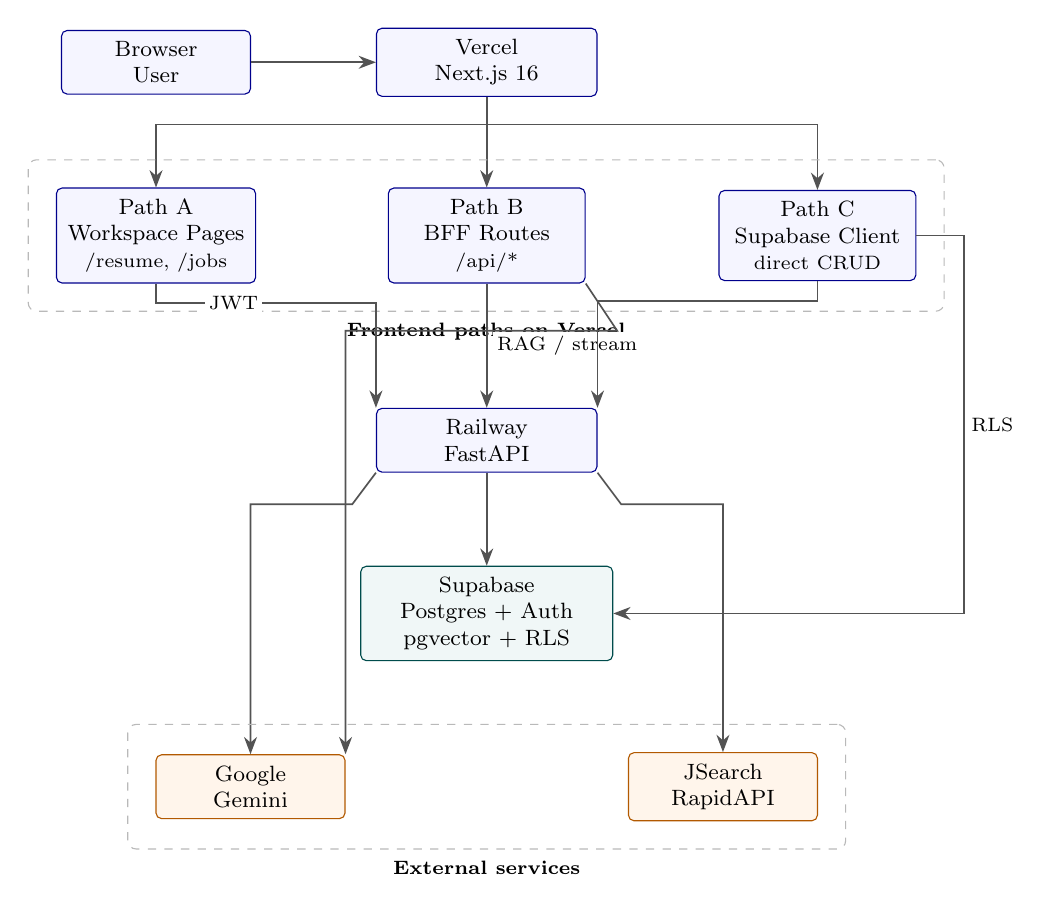
\begin{tikzpicture}[
  x=1cm, y=1cm,
  every node/.style={align=center},
]
  % Row 1 — entry
  \node[flowbox, minimum width=2.4cm] (user) at (0,0) {Browser\\User};
  \node[flowbox, minimum width=2.8cm] (vercel) at (4.2,0) {Vercel\\Next.js 16};

  \draw[arr] (user) -- (vercel);

  % Row 2 — three frontend paths
  \node[flowbox, minimum width=2.5cm] (pathA) at (0,-2.2) {Path A\\Workspace Pages\\{\scriptsize /resume, /jobs}};
  \node[flowbox, minimum width=2.5cm] (pathB) at (4.2,-2.2) {Path B\\BFF Routes\\{\scriptsize /api/*}};
  \node[flowbox, minimum width=2.5cm] (pathC) at (8.4,-2.2) {Path C\\Supabase Client\\{\scriptsize direct CRUD}};

  \draw[arr] (vercel.south) -- ++(0,-0.35) -| (pathA.north);
  \draw[arr] (vercel.south) -- (pathB.north);
  \draw[arr] (vercel.south) -- ++(0,-0.35) -| (pathC.north);

  \node[groupbox, fit=(pathA)(pathB)(pathC), inner sep=10pt] (febox) {};
  \node[grouplabel, below=2pt of febox.south] {Frontend paths on Vercel};

  % Row 3 — backend hub
  \node[flowbox, minimum width=2.8cm] (api) at (4.2,-4.8) {Railway\\FastAPI};

  \draw[arr] (pathA.south) -- ++(0,-0.25) -| node[lbl, near start, left=1pt] {JWT} (api.north west);
  \draw[arr] (pathB.south) -- node[lbl, right=2pt] {RAG / stream} (api.north);
  \draw[arr] (pathC.south) -- ++(0,-0.25) -| (api.north east);

  % Row 4 — data store
  \node[databox, minimum width=3.2cm] (supa) at (4.2,-7.0) {Supabase\\Postgres + Auth\\pgvector + RLS};

  \draw[arr] (api) -- (supa);
  \draw[arr] (pathC.east) -- ++(0.6,0) |- node[lbl, pos=0.25, right=1pt] {RLS} (supa.east);

  % Row 5 — external services
  \node[extbox, minimum width=2.4cm] (gemini) at (1.2,-9.2) {Google\\Gemini};
  \node[extbox, minimum width=2.4cm] (jsearch) at (7.2,-9.2) {JSearch\\RapidAPI};

  \draw[arr] (api.south west) -- ++(-0.3,-0.4) -| (gemini.north);
  \draw[arr] (pathB.south east) -- ++(0.4,-0.6) -| (gemini.north east);
  \draw[arr] (api.south east) -- ++(0.3,-0.4) -| (jsearch.north);

  \node[groupbox, fit=(gemini)(jsearch), inner sep=10pt] (extgroup) {};
  \node[grouplabel, below=2pt of extgroup.south] {External services};
\end{tikzpicture}%
}
\end{center}

\vspace{0.4em}
{\footnotesize
\textbf{Path A} (FastAPI): CV ingest, job search, fit scoring, tracker --- Bearer JWT to Railway.\\
\textbf{Path B} (BFF): LLM streaming for chat, cover letters, roadmaps, dashboard nudges.\\
\textbf{Path C} (Direct): Calendar events and standalone tasks --- Supabase anon key + RLS.
}

% --- Figure 2: CV / RAG ----------------------------------------------------
\newpage
\flowtitle{Figure 2 --- CV Upload \& RAG Core (Single Source of Truth)}

\begin{center}
\adjustbox{max width=\linewidth}{%
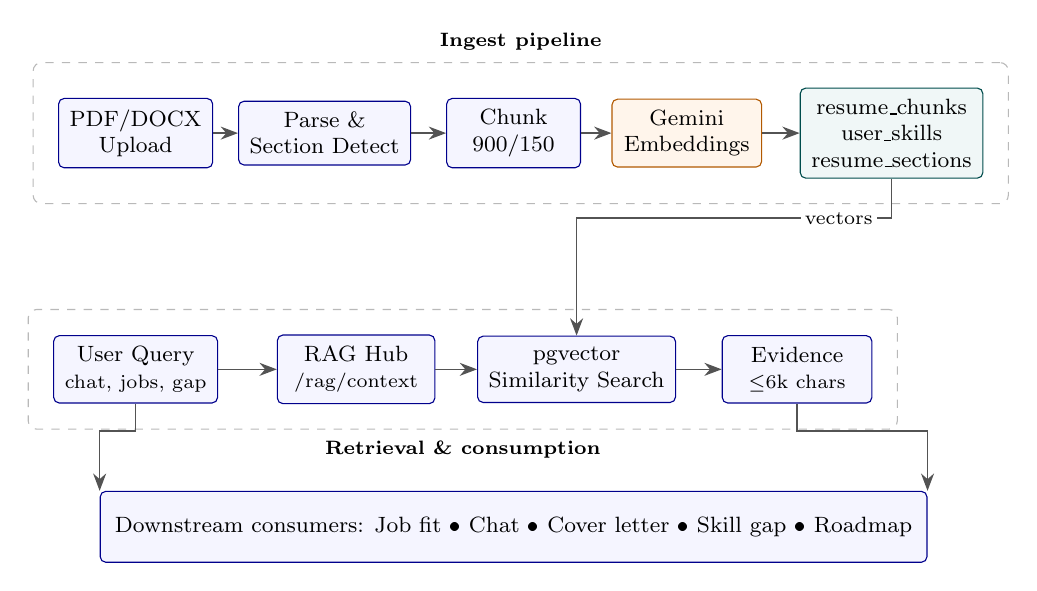
\begin{tikzpicture}[
  x=1cm, y=1cm,
  every node/.style={align=center},
]
  % --- Ingest pipeline (top, left-to-right) ---
  \node[flowbox, minimum width=1.9cm] (upload) at (0,0) {PDF/DOCX\\Upload};
  \node[flowbox, minimum width=1.9cm] (parse)  at (2.4,0) {Parse \&\\Section Detect};
  \node[flowbox, minimum width=1.7cm] (chunk)  at (4.8,0) {Chunk\\900/150};
  \node[extbox,  minimum width=1.9cm] (embed)  at (7.0,0) {Gemini\\Embeddings};
  \node[databox, minimum width=2.2cm] (store)  at (9.6,0) {resume\_chunks\\user\_skills\\resume\_sections};

  \draw[arr] (upload) -- (parse);
  \draw[arr] (parse) -- (chunk);
  \draw[arr] (chunk) -- (embed);
  \draw[arr] (embed) -- (store);

  \node[groupbox, fit=(upload)(parse)(chunk)(embed)(store), inner sep=9pt] (ingest) {};
  \node[grouplabel, above=2pt of ingest.north] {Ingest pipeline};

  % --- Retrieval pipeline (middle, left-to-right) ---
  \node[flowbox, minimum width=2.0cm] (query) at (0,-3.0) {User Query\\{\scriptsize chat, jobs, gap}};
  \node[flowbox, minimum width=2.0cm] (rag)   at (2.8,-3.0) {RAG Hub\\{\scriptsize /rag/context}};
  \node[flowbox, minimum width=2.0cm] (retrieve) at (5.6,-3.0) {pgvector\\Similarity Search};
  \node[flowbox, minimum width=1.9cm] (evidence) at (8.4,-3.0) {Evidence\\{\scriptsize $\leq$6k chars}};

  \draw[arr] (query) -- (rag);
  \draw[arr] (rag) -- (retrieve);
  \draw[arr] (retrieve) -- (evidence);
  \draw[arr] (store.south) -- ++(0,-0.5) -| node[lbl, pos=0.15, right=1pt] {vectors} (retrieve.north);

  \node[groupbox, fit=(query)(rag)(retrieve)(evidence), inner sep=9pt] (retr) {};
  \node[grouplabel, below=2pt of retr.south] {Retrieval \& consumption};

  % --- Downstream consumers (bottom) ---
  \node[flowbox, minimum width=10.5cm, minimum height=0.9cm] (consumers) at (4.8,-5.0)
    {Downstream consumers: Job fit \textbullet\ Chat \textbullet\ Cover letter \textbullet\ Skill gap \textbullet\ Roadmap};

  \draw[arr] (evidence.south) -- ++(0,-0.35) -| (consumers.north east);
  \draw[arr] (query.south) -- ++(0,-0.35) -| (consumers.north west);
\end{tikzpicture}%
}
\end{center}

% --- Figure 3: Job search --------------------------------------------------
\newpage
\flowtitle{Figure 3 --- Job Search \& Fit Scoring Data Flow}

\begin{center}
\adjustbox{max width=\linewidth}{%
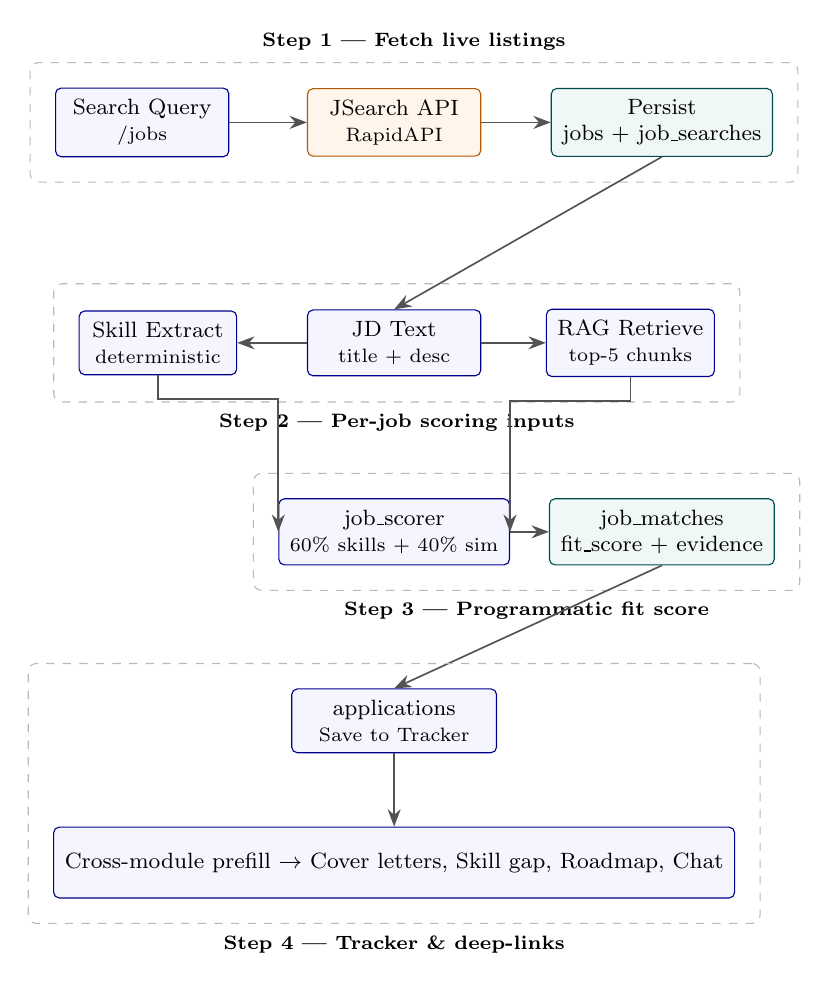
\begin{tikzpicture}[
  x=1cm, y=1cm,
  every node/.style={align=center},
]
  % Row 1 — fetch listings
  \node[flowbox, minimum width=2.2cm] (search) at (0,0) {Search Query\\{\scriptsize /jobs}};
  \node[extbox,  minimum width=2.2cm] (js)     at (3.2,0) {JSearch API\\{\scriptsize RapidAPI}};
  \node[databox, minimum width=2.4cm] (jobs)   at (6.6,0) {Persist\\jobs + job\_searches};

  \draw[arr] (search) -- (js);
  \draw[arr] (js) -- (jobs);

  \node[groupbox, fit=(search)(js)(jobs), inner sep=9pt] (fetch) {};
  \node[grouplabel, above=2pt of fetch.north] {Step 1 --- Fetch live listings};

  % Row 2 — per-job scoring inputs
  \node[flowbox, minimum width=2.2cm] (jd)     at (3.2,-2.8) {JD Text\\{\scriptsize title + desc}};
  \node[flowbox, minimum width=2.0cm] (skills) at (0.2,-2.8) {Skill Extract\\{\scriptsize deterministic}};
  \node[flowbox, minimum width=2.0cm] (ragj)   at (6.2,-2.8) {RAG Retrieve\\{\scriptsize top-5 chunks}};

  \draw[arr] (jobs.south) -- (jd.north);
  \draw[arr] (jd.west) -- (skills.east);
  \draw[arr] (jd.east) -- (ragj.west);

  \node[groupbox, fit=(skills)(jd)(ragj), inner sep=9pt] (inputs) {};
  \node[grouplabel, below=2pt of inputs.south] {Step 2 --- Per-job scoring inputs};

  % Row 3 — score and persist
  \node[flowbox, minimum width=2.4cm] (score) at (3.2,-5.2)
    {job\_scorer\\{\scriptsize 60\% skills + 40\% sim}};
  \node[databox, minimum width=2.4cm] (match) at (6.6,-5.2)
    {job\_matches\\fit\_score + evidence};

  \draw[arr] (skills.south) -- ++(0,-0.3) -| (score.west);
  \draw[arr] (ragj.south) -- ++(0,-0.3) -| (score.east);
  \draw[arr] (score) -- (match);

  \node[groupbox, fit=(score)(match), inner sep=9pt] (scorebox) {};
  \node[grouplabel, below=2pt of scorebox.south] {Step 3 --- Programmatic fit score};

  % Row 4 — tracker + cross-module
  \node[flowbox, minimum width=2.6cm] (tracker) at (3.2,-7.6)
    {applications\\{\scriptsize Save to Tracker}};
  \node[flowbox, minimum width=5.8cm, minimum height=0.9cm] (xmod) at (3.2,-9.4)
    {Cross-module prefill $\rightarrow$ Cover letters, Skill gap, Roadmap, Chat};

  \draw[arr] (match.south) -- (tracker.north);
  \draw[arr] (tracker) -- (xmod);

  \node[groupbox, fit=(tracker)(xmod), inner sep=9pt] (trackbox) {};
  \node[grouplabel, below=2pt of trackbox.south] {Step 4 --- Tracker \& deep-links};
\end{tikzpicture}%
}
\end{center}

% --- Figure 4: Assistant & generation --------------------------------------
\newpage
\flowtitle{Figure 4 --- Assistant Chat \& Career Artifact Generation}

\begin{center}
\adjustbox{max width=\linewidth}{%
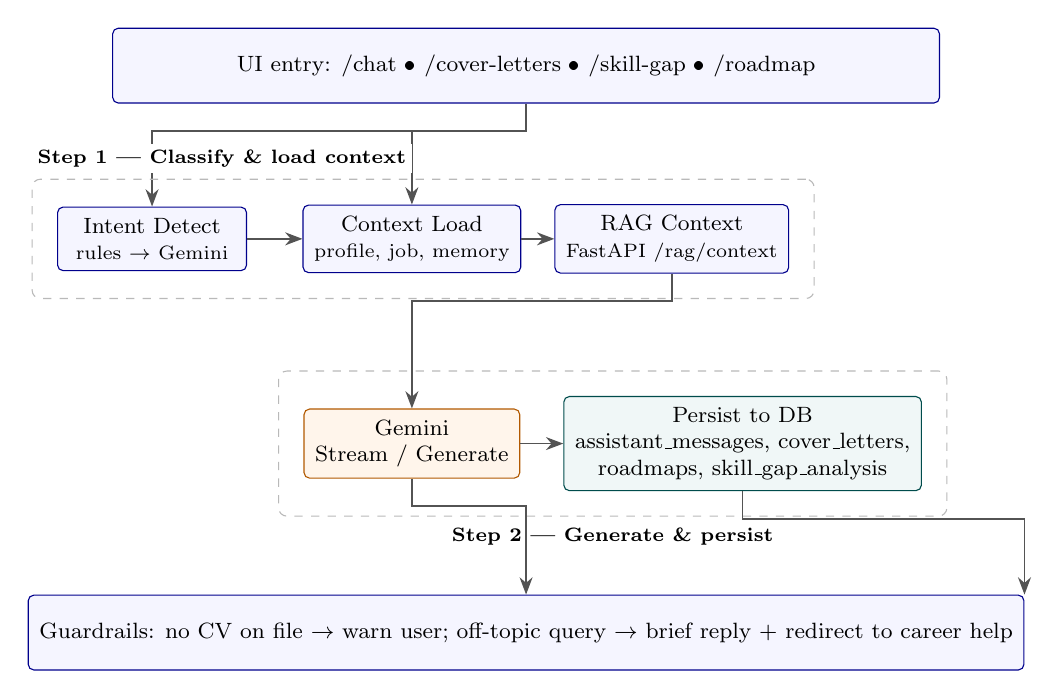
\begin{tikzpicture}[
  x=1cm, y=1cm,
  every node/.style={align=center},
]
  % Row 1 — UI entry points
  \node[flowbox, minimum width=10.5cm, minimum height=0.95cm] (ui) at (5.25,0)
    {UI entry: /chat \textbullet\ /cover-letters \textbullet\ /skill-gap \textbullet\ /roadmap};

  % Row 2 — preprocessing chain
  \node[flowbox, minimum width=2.4cm] (intent) at (0.5,-2.2) {Intent Detect\\{\scriptsize rules $\rightarrow$ Gemini}};
  \node[flowbox, minimum width=2.4cm] (ctx)    at (3.8,-2.2) {Context Load\\{\scriptsize profile, job, memory}};
  \node[flowbox, minimum width=2.4cm] (ragc)   at (7.1,-2.2) {RAG Context\\{\scriptsize FastAPI /rag/context}};

  \draw[arr] (ui.south) -- ++(0,-0.35) -| (intent.north);
  \draw[arr] (ui.south) -- ++(0,-0.35) -| (ctx.north);
  \draw[arr] (intent) -- (ctx);
  \draw[arr] (ctx) -- (ragc);

  \node[groupbox, fit=(intent)(ctx)(ragc), inner sep=9pt] (pre) {};
  \node[grouplabel, above=2pt of pre.north west, anchor=south west] {Step 1 --- Classify \& load context};

  % Row 3 — generation
  \node[extbox, minimum width=2.4cm] (gem) at (3.8,-4.8) {Gemini\\Stream / Generate};
  \node[databox, minimum width=3.2cm] (persist) at (8.0,-4.8)
    {Persist to DB\\assistant\_messages, cover\_letters,\\roadmaps, skill\_gap\_analysis};

  \draw[arr] (ragc.south) -- ++(0,-0.35) -| (gem.north);
  \draw[arr] (gem) -- (persist);

  \node[groupbox, fit=(gem)(persist), inner sep=9pt] (gen) {};
  \node[grouplabel, below=2pt of gen.south] {Step 2 --- Generate \& persist};

  % Row 4 — guardrails
  \node[flowbox, minimum width=10.5cm, minimum height=0.95cm] (guard) at (5.25,-7.2)
    {Guardrails: no CV on file $\rightarrow$ warn user; off-topic query $\rightarrow$ brief reply + redirect to career help};

  \draw[arr] (gem.south) -- ++(0,-0.35) -| (guard.north);
  \draw[arr] (persist.south) -- ++(0,-0.35) -| (guard.north east);
\end{tikzpicture}%
}
\end{center}

% ===========================================================================
\newpage
\sectiontitle{2. Scaling Analysis (10{,}000 Users)}
% ===========================================================================

\noindent
\textbf{Planning assumption:} 10{,}000 monthly active users (MAU), moderate usage
(1 CV upload, 3 job searches, 5 chat turns, 2 AI workflows per user/month).

\vspace{0.6em}
\noindent
\fbox{%
  \parbox{\dimexpr\linewidth-2\fboxsep-2\fboxrule}{%
    \textbf{Current architecture supports approximately 500 concurrent users.}\\[0.4em]
    At peak, a single Railway FastAPI instance, Vercel serverless concurrency limits,
    synchronous CV processing, and Supabase connection caps bound throughput before
    horizontal scaling, async workers, and shared caching are applied.
  }%
}

\vspace{0.8em}
\noindent\textbf{To support 10{,}000 users:}

\begin{enumerate}[leftmargin=*, itemsep=3pt]
  \item \textbf{Async CV processing} --- Move parse $\rightarrow$ chunk $\rightarrow$ embed off the upload request path; enqueue to Upstash Redis; Railway worker updates \texttt{resumes.status}; frontend polls or uses realtime.
  \item \textbf{Horizontal API scaling} --- Run 3--4 stateless FastAPI instances on Railway behind a load balancer; JWT carries identity (no sticky sessions).
  \item \textbf{Database tier upgrade} --- Supabase Pro with connection pooler (transaction mode for serverless, session mode for workers); covering indexes on \texttt{applications(user\_id)}, \texttt{job\_matches(user\_id)}, \texttt{resume\_chunks(user\_id)}.
  \item \textbf{Centralize AI calls} --- Route all Gemini traffic through FastAPI (or a dedicated AI gateway); enforce per-user daily quotas; default to Flash-class models.
  \item \textbf{Shared cache layer} --- Replace in-memory nudge \texttt{Map} with Upstash Redis (TTL 15--60\,min); cache JSearch \texttt{(query, location)} responses.
  \item \textbf{Vector index evolution} --- Keep IVFFlat for $<$50k chunks; migrate to HNSW when \texttt{resume\_chunks} exceeds ${\sim}$500k rows; align embedding dimension across config, column, and RPC.
  \item \textbf{Job deduplication} --- Unique constraint on \texttt{(source, source\_url)} with upsert to prevent storage bloat from repeat searches.
  \item \textbf{Vercel Pro tuning} --- Extended serverless timeouts (60s+) for chat/nudge BFF routes; React Query staleTime to reduce dashboard re-fetches.
  \item \textbf{Observability} --- Request IDs across BFF $\rightarrow$ FastAPI; metrics for p95 RAG latency, Gemini token usage, JSearch 429 rate.
  \item \textbf{Scheduled reminders} --- Add cron / workflow service (Supabase Edge Functions, Inngest) for calendar \texttt{reminder\_time} delivery.
\end{enumerate}

\vspace{0.5em}
\noindent
{\footnotesize
\textbf{Traffic at 10k MAU (planning):}
${\sim}$10k CV uploads \textbullet\ ${\sim}$30k JSearch calls \textbullet\
${\sim}$50k chat turns \textbullet\ ${\sim}$20k generation workflows \textbullet\
${\sim}$200k lightweight DB reads.
}

\newpage

% ===========================================================================
\sectiontitle{3. Estimated Cost per User / Month}
% ===========================================================================

\noindent
Planning estimates from public pricing (June 2026). Not billing guarantees.
Moderate AI usage profile at 10{,}000 MAU.

\vspace{0.5em}
\begin{center}
\small
\renewcommand{\arraystretch}{1.35}
\begin{tabularx}{\linewidth}{|l|>{\raggedright\arraybackslash}X|>{\raggedleft\arraybackslash}r|}
\hline
\textbf{Component} & \textbf{Planning choice} & \textbf{Est.\ USD/mo} \\
\hline
Backend API       & Railway (2 web services + 1 worker)         & \$45--\$80 \\
\hline
Queue             & Upstash Redis (pay-as-you-go)               & \$10 \\
\hline
Database / Auth / Vector & Supabase Pro (+ modest compute)      & \$75 \\
\hline
Job search        & JSearch Pro / Ultra (30k searches/mo)        & \$30--\$75 \\
\hline
Gemini AI         & Embeddings + generation (moderate usage)     & \$25--\$120 \\
\hline
Frontend (ref.)   & Vercel Pro                                   & \$20 \\
\hline
Observability     & Logs, overages, storage buffer               & \$15--\$25 \\
\hline
\textbf{Total}    &                                              & \textbf{\$220--\$405} \\
\hline
\end{tabularx}
\end{center}

\costheading{Cost per active user per month:}
\formulabox{%
  $\begin{aligned}
    C_{\text{user}}
      &= \frac{C_{\text{fixed}} + C_{\text{Gemini}} + C_{\text{JSearch\_overage}}}{N_{\text{MAU}}} \\
    &\approx \frac{\$220\text{--}\$405}{10{,}000} \\
    &\approx \mathbf{\$0.022\text{--}\$0.041 \;/\; \text{user / month}}
  \end{aligned}$%
}
\noindent Rounded planning figure: \textbf{${\sim}\$0.03$ per MAU per month} at moderate usage.

\costheading{Variable Cost Drivers (Formulas)}

\noindent\textbf{JSearch:}
\formulabox{%
  $\begin{aligned}
    R &= N_{\text{MAU}} \times s_{\text{user}} \\
    &\text{(e.g.\ } R = 10{,}000 \times 3 = 30{,}000 \text{ req/mo)} \\[0.2em]
    C_{\text{JSearch}} &= P_{\text{plan}} + \max(0,\; R - R_{\text{included}}) \times r_{\text{overage}}
  \end{aligned}$%
}

\noindent\textbf{Gemini embeddings:}
\formulabox{%
  $C_{\text{embed}} = \dfrac{T_{\text{CV}} + T_{\text{query}}}{10^{6}} \times p_{\text{embed}}$%
}

\noindent\textbf{Gemini generation:}
\formulabox{%
  $\begin{aligned}
    C_{\text{gen}} &= \frac{T_{\text{in}}}{10^{6}} \times p_{\text{in}} \\
                   &\quad + \frac{T_{\text{out}}}{10^{6}} \times p_{\text{out}}
  \end{aligned}$%
}

\noindent\textbf{Total variable AI:}
\formulabox{%
  $C_{\text{Gemini}} = C_{\text{embed}} + C_{\text{gen}}$%
}
\noindent
where $T$ = tokens, $p$ = per-million rates from Gemini pricing.
At 10 AI workflows/user/month, $C_{\text{Gemini}}$ can exceed \$120 and dominate total cost.

\noindent\textbf{Per-user total:}
\formulabox{%
  $C_{\text{user}} = \dfrac{C_{\text{fixed}} + C_{\text{Gemini}} + C_{\text{JSearch}}}{N_{\text{MAU}}}$%
}

% ===========================================================================
\newpage
\sectiontitle{4. Key Bottlenecks and Mitigations}
% ===========================================================================

{\footnotesize
\begin{longtable}{@{}p{5mm} p{22mm} p{30mm} p{32mm} p{32mm}@{}}
\toprule
\textbf{\#} & \textbf{Bottleneck} & \textbf{Risk at Scale} & \textbf{Evidence in Codebase} & \textbf{Mitigation} \\
\midrule
\endhead

1 &
AI API Usage (Gemini) &
Many features rely on Gemini. As user numbers grow, API costs and rate limits may become a problem. &
Gemini is used for chat, resume analysis, cover letters, interview preparation, roadmaps, and skill-gap analysis. &
Add daily usage limits per user, cache repeated requests, and use lower-cost Gemini models where possible. \\[2pt]

2 &
Resume Processing During Upload &
Upload requests take longer because resume parsing, embedding generation, and database updates happen immediately. Multiple uploads at once could slow the system. &
Resume processing runs directly during the upload request. &
Move processing to a background worker and notify users when processing is complete. \\[2pt]

3 &
Job Search API Dependency &
If the external Job Search API becomes slow or reaches its quota limit, job recommendations may stop working. &
All job searches depend on the JSearch API. &
Cache search results, reduce duplicate searches, and upgrade the API plan if needed. \\[2pt]

4 &
Multiple AI Entry Points &
AI requests are handled from several different places, making monitoring and rate limiting difficult. &
Both FastAPI and Next.js routes communicate with Gemini. &
Route all AI requests through a single backend service. \\[2pt]

5 &
In-Memory Cache &
Cached data is stored only on one server instance. In a multi-server deployment, users may receive inconsistent results. &
Nudge cache currently uses an in-memory Map. &
Replace with Redis or another shared cache system. \\[2pt]

6 &
Vector Search Growth &
As more resumes are stored, similarity search may become slower and less accurate. &
Resume embeddings are stored using pgvector. &
Upgrade indexing strategy and archive old data when necessary. \\[2pt]

7 &
Database Connection Limits &
Many simultaneous users may exceed the database's connection limit. &
Multiple services create database connections independently. &
Use connection pooling and limit unnecessary database requests. \\[2pt]

8 &
Duplicate Job Listings &
Repeated job searches can store the same job multiple times, increasing storage usage. &
Job records are inserted without strong duplicate checking. &
Add unique constraints and use upsert operations. \\[2pt]

9 &
Reminder Delivery &
Reminder times are stored, but notifications are not automatically sent to users. &
Reminder data exists but no scheduler is configured. &
Add scheduled jobs using cron or a workflow service. \\[2pt]

10 &
Limited Monitoring &
Production issues may be difficult to diagnose due to limited monitoring and metrics collection. &
Basic logging exists, but no centralized monitoring. &
Add metrics, request tracing, and performance dashboards. \\[2pt]

11 &
File Storage Reliability &
If a resume file upload fails silently, the resume cannot be processed later. &
Storage upload errors are not always enforced. &
Verify file uploads before marking resumes as successfully processed. \\[2pt]

12 &
Job Matching Computation &
Every job search performs scoring calculations for many jobs, increasing CPU usage. &
Job matching is performed for each returned job. &
Limit the number of jobs scored and precompute frequently used embeddings. \\

\bottomrule
\end{longtable}
}

% ===========================================================================
\section*{5. Highest-Priority Fixes Before Production}
% ===========================================================================

\begin{enumerate}[leftmargin=*, itemsep=4pt]
  \item Move resume processing to an asynchronous background worker.
  \item Centralize all Gemini API calls and add per-user usage limits.
  \item Replace the in-memory cache with Redis.
  \item Verify embedding/vector configuration consistency.
  \item Add caching for external job search API responses.
\end{enumerate}

\vspace{1em}
\hrule
\vspace{0.4em}
{\footnotesize
\textit{CareerPilot System Design --- derived from \texttt{Docs/submit/system-design.md}.}\\
Pricing refs: \url{https://railway.app/pricing} \textbullet\
\url{https://supabase.com/pricing} \textbullet\
\url{https://ai.google.dev/pricing} \textbullet\
\url{https://upstash.com/pricing} \textbullet\
JSearch via RapidAPI.
}

\end{document}
